%% DONE
\id{IRSTI 47.09.48}{}

\begin{articleheader}
\sectionwithauthors{D.B. Konarbay, Y. Bakytkarim, Zh.S. Mukataeva, N.A. Shadin, D.A. Karazhanova, Zh.R. Kozhagulova}{IMPORTANCE OF MXENE NANOCOMPOSITES IN THE DETECTION OF HEAVY METALS}

{\bfseries D.B. Konarbay\textsuperscript{\envelope } \authorid,
Y. Bakytkarim\textsuperscript{\envelope } \authorid,
Zh.S. Mukataeva\authorid,
N.A. Shadin\authorid,
D.A. Karazhanova\authorid,
Zh.R. Kozhagulova\authorid}
\end{articleheader}

\begin{affiliation}
\emph{Abai Kazakh National Pedagogical University», Almaty city, Kazakhstan}

\raggedright \textsuperscript{\envelope }{\em Corresponding-author: \emph{\href{mailto:konarbay98@bk.ru}{\nolinkurl{konarbay98@bk.ru}}, \href{mailto:Rysgul_01_88@mail.ru}{\nolinkurl{Rysgul\_01\_88@mail.ru}}}}
\end{affiliation}

One of the strongest and most common chemical pollution is its
environmental pollution with heavy metals. Heavy metals are actively
involved in biological processes, which are part of many enzymes. The
toxicity of heavy metal ions causes a number of harm to environmental
components and human health. That is why the detection of heavy metals
is so important. The creation of a reliable and effective system for
detecting heavy metals is crucial. And traditional detection methods are
often not enough to meet the current needs. Therefore, the use of
electrochemical sensors in the detection of heavy metals is currently
taking an important place. Electrochemical sensors have become a
promising area of research due to their unique capabilities. Improving
the detection efficiency of electrochemical sensors is the main area of
research. The leading strategy for significantly improving detection
performance involves adding nanomaterials to electrochemical sensors.
This review compares MXene nanocompasites with the achievements of
nanomaterials in the field of electrochemical sensors in recent years.
This makes it possible to obtain new ideas for the manufacture of
electrochemical sensors with high sensitivity and low detection
threshold. We believe that knowing and combining the benefits of
different nanomaterials to produce innovative electrode modification
materials can eliminate the risk of heavy metal ions in many food,
environmental and other industries.

{\bfseries Keywords:} heavy metals, electrochemical sensors, nanomaterials,
modification, MXene nanocomposites.

\begin{articleheader}
{\bfseries АУЫР МЕТАЛДАРДЫ АНЫҚТАУДА MXENE НАНОКОМПОЗИТТЕРДІҢ МАҢЫЗЫ}

{\bfseries
Д.Б. Қонарбай\textsuperscript{\envelope },
Ы. Бақыткәрім\textsuperscript{\envelope },
Ж.С. Мұқатаева,
Н.А. Шадин
Д.А. Каражанова,
Ж.Р. Кожагулова}
\end{articleheader}

\begin{affiliation}
\emph{Абай атындағы Қазақ ұлттық педагогикалық университеті», Алматы, Қазақстан,}

e-mail: \emph{\href{mailto:konarbay98@bk.ru}{\nolinkurl{konarbay98@bk.ru}}, \href{mailto:Rysgul_01_88@mail.ru}{\nolinkurl{Rysgul\_01\_88@mail.ru}}}
\end{affiliation}

Ең күшті және ең көп таралған химиялық ластанудың бірі - ол қоршаған
ортаның ауыр металдармен ластануы. Ауыр металдар көптеген ферменттердің
құрамына кіретін биологиялық процестерге белсенді қатысады. Ауыр металл
иондарының уыттылығы қоршаған орта компоненттеріне және адам
денсаулығына бірқатар зиянын келтіреді. Сондықтан да ауыр металдарды
анықтау өте маңызды болып табылады. Ауыр металдарды анықтау үшін сенімді
және тиімді жүйені құру қажет. Ал дәстүрлі анықтау әдістері көбінесе
қазіргі қажеттіліктерді қанағаттандыру үшін жеткіліксіз. Сондықтанда
қазіргі кезде ауыр металдарды анықтауда электрохимиялық сенсорларды
қолдану маңызды орын алып отыр. Электрохимиялық сенсорлар өзінің ерекше
мүмкіндіктерінің арқасында зерттеудің перспективалық бағытына айналды.
Электрохимиялық сенсорларды анықтау тиімділігін арттыру зерттеудің
негізгі бағыты болып табылады. Анықтау өнімділігін айтарлықтай
жақсартудың жетекші стратегиясы наноматериалдарды электрохимиялық
сенсорларға қосуды қамтиды. Бұл шолу MXene нанокомпазиттерін
соңғы жылдардағы электрохимиялық сенсорлар саласындағы
наноматериалдардың жетістіктерін салыстырады. Бұл жоғары
сезімталдығы бар және анықтау шегі төмен электрохимиялық
сенсорларды дайындау үшін жаңа идеялар алуға мүмкіндік береді.
Электродтарды модификациялау үшін инновациялық материалдар алу
үшін әртүрлі наноматериалдардың артықшылықтарын білу және
біріктіру көптеген азық-түлік, экологиялық және де басқа
салалардағы ауыр металл иондарының қаупін жоя алады деген
ойдамыз.

{\bfseries Түйін сөздер:} Ауы{\bfseries }р металдар, электрохимиялық
сенсорлар, наноматериалдар, модификация, MXene нанокомпозиттері.

\begin{articleheader}
{\bfseries ВАЖНОСТЬ НАНОКОМПОЗИТОВ MXENE ДЛЯ ОПРЕДЕЛЕНИЯ ТЯЖЕЛЫХ МЕТАЛЛОВ}

{\bfseries Д.Б. Конарбай\textsuperscript{\envelope },
Ы. Бакыткарим\textsuperscript{\envelope },
Ж.С. Мукатаева,
Н.А.Шадин,
Д.А. Каражанова,
Ж.Р. Кожагулова}
\end{articleheader}

\begin{affiliation}
\emph{Казахский национальный педагогический университет имени Абая», г. Алматы, Казахстан,}

\emph{e-mail: \href{mailto:konarbay98@bk.ru}{\nolinkurl{konarbay98@bk.ru}}, \href{mailto:Rysgul_01_88@mail.ru}{Rysgul\_01\_88@mail.ru}}
\end{affiliation}

Одним из самых сильных и распространенных химических загрязнений
является загрязнение окружающей среды тяжелыми металлами. Тяжелые
металлы активно участвуют в биологических процессах, входя в
состав многих ферментов. Токсичность ионов тяжелых металлов
наносит ряд повреждений компонентам окружающей среды и здоровью
человека. Именно поэтому обнаружение тяжелых металлов так важно.
Необходимо создать надежную и эффективную систему для обнаружения
тяжелых металлов. А традиционных методов обнаружения зачастую
недостаточно для удовлетворения современных потребностей. Поэтому
использование электрохимических сенсоров для обнаружения тяжелых
металлов в настоящее время занимает важное место.
Электрохимические сенсоры стали перспективным направлением
исследований благодаря своим уникальным возможностям. Повышение
эффективности обнаружения электрохимических сенсоров является
основным направлением исследований. Ведущей стратегией для
значительного повышения эффективности обнаружения является
добавление наноматериалов в электрохимические сенсоры. В данном
обзоре сравниваются нанокомпозиты MXene с достижениями
наноматериалв в области электрохимических сенсоров за последние
годы. Это позволяет получить новые идеи для изготовления
электрохимических сенсоров с выской чувствительностью и низким
порогом обнаружения. Мы считаем, что знание и комбинирование
преимуществ различных наноматериалов для создания инновационных
материалов для модификации электродов может устранить опасность
ионов тяжелых металлов во многих пищевых, экологических и других
отраслях промышленности.

{\bfseries Ключевые слова:} тяжелые металлы, электрохимические
сенсоры, наноматериалы, модификация, нанокомпозиты MXene.

\begin{multicols}{2}
{\bfseries Introduction.} Heavy metals are particularly biodegradable
pollutants. They enter aquatic ecosystems, enter water and
sediment phases, accumulate in organisms, and even at low levels
cause a number of serious diseases and disorders {[}1-4{]}. For
example, neurological, cardiovascular, respiratory and
reproductive diseases {[}5{]}. Heavy metals in the environment
pose a serious threat to wildlife and human health because they
are bioavailable and can be absorbed and enriched in food
{[}6{]}. Toxic metals are largely distributed into the
environment. The distribution of heavy metals by wind in the
form of particles or vapor depends on their physical state. The
meta-components move from the atmosphere to the soil or water
surface, resulting in environmental pollution. Industrial
wastewater is a major source of metal pollution in the
hydrosphere. Wastewater containing toxic heavy metals like
nickel, lead, copper, chromium, cadmium, and arsenic poses
environmental and health hazards {[}7{]}. Heavy metals affecting
human health include elements such as mercury, nickel, lead,
chromium, cadmium, aluminum and copper {[}8{]}. Heavy metals in
water, air and soil can be transferred to plants, aquatic
organisms and organisms and then enter the food chain and
pose a threat to human health {[}9{]}.

Year after year, the population around the world is growing. As
the world' s population grows, the demand for
food, drinking water and many other industries increases. Due
to the increased demand, the quality requirements for food and
drinking water are increasing. To ensure consumer safety, we
must detect harmful substances present in very low
concentrations. One of the most commonly used methods today is
the use of electrochemical sensors.

Electrochemical sensors are tools for detecting and counting
heavy metals because they tend to be highly specific, sensitive,
inexpensive and portable. This makes them valuable for small
and mobile remote applications. Since complete elimination of
food and drinking water contamination may not seem possible in
the near future, assessment of legal limits should always be
considered in the context of general nutrition, especially in the
case of children. Ongoing research continues to improve sensor
performance, enhance detection capabilities, and address
calibration, interference, and sample preparation issues, further
advancing the development of electrochemical sensors in food
safety applications {[}10{]}.

The world of sensors is diverse and due to this, it is developing
at a rapid pace. Due to continuous technological improvement it is
becoming more and more in demand. Electrochemical sensors are a
convenient solution for variable analyzer detection due to their
low cost and availability and are widely used in agriculture,
food and oil industry as well as in environmental and biomedical
fields. Electrochemical sensors have long been required for the
study of biological substances. The sensors are characterized
not only by their durability, high sensitivity and accuracy,
but also by their low cost, speed and simplicity. Many
nanomaterials have been obtained in more than two decades.
Specific metals, conducting polymers, metal oxides and
organometallic and carbon-based nanomaterial structures.
Nanomaterials contribute to the analytical performance included in
electrochemical analysis. This modification increases the payload
capacity by utilizing recognition molecules such as enzymes,
antibodies and aptamers as well as bioinspired receptors that
can accurately and efficiently capture the target, thereby
increasing the specificity of electrochemical sensors {[}11{]}.
\end{multicols}

\begin{table}[H]
\caption*{Table 1 - Lists many MXene-based sensors and their corresponding applications {[}19{]}}
\centering
\begin{tblr}{
  colspec = {X[1] X[1]},
  row{1} = {c},
  hlines,
  vlines,
}
Nanocomposite components                              & Application                                            \\
Ti$_3$C$_2$ / reduced graphene oxide                    & Pressure sensor                                       \\
Ti$_3$C$_2$/ Ag nanowire                                  & Strain sensor                                         \\
Ti$_3$C$_2$ / chitosan                                    & Biosensor for detecting pesticides                  \\
Ti$_3$C$_2$ / Nafion                                      & Detecting nitrile ions                               \\
Ti$_3$C$_2$ / PANI                                        & Ethanol, methanol, ammonia, and acetone detection \\
Ti$_3$C$_2$ / polyurethane                                & Stretchable strain sensing fabric                   \\
Ti$_3$C$_2$/ poly(vinylidene fluoride-trifluoroethylene)  & Capacitive pressure sensor                           \\
Ti$_3$C$_2$ / natural microcapsules                       & Epidermal flexible pressure sensors                 \\
Ti$_3$C$_2$ / poly(dimethylsiloxane)                      & Skin conformal sensors for health monitoring      \\
Ti$_3$C$_2$ / gold nanoparticles                          & Glucose detection biosensor                          \\
Ti$_3$C$_2$ and TiO$_2$                                   & H$_2$O$_2$ detection                                      \\
hollow MXene spheres/ reduced graphene                   & Piezoresistive pressure sensor                       \\
Ti$_3$C$_2$ / ink                                         & Strain sensor for health monitoring                
\end{tblr}
\end{table}

\begin{multicols}{2}
Electrochemistry-an important quantitative analysis strategy for
testing various biochemical entities such as proteins,
metabolites, neurotransmitters, electrolytes, heavy metals, etc.
Further, demonstrating wide applications in the fields of private
health care, public health, clinical diagnostics, food safety
and environmental analysis {[}12-14{]}. Generally, a complete
electrochemical conversion system usually consists of two parts:
sensing electrodes and electrochemically sensitive circuits. The
former is used to convert biochemical signals into electrical
signals. The latter uses various electrochemical test methods to
excite the electrodes with voltage, collect, process, analyze
the data and transmit them as electrical signals {[}15,16{]}.

MXenes'{} electrical conductivity, rich surface
chemistry and high aspect ratio are attractive characteristics
for sensor processing . The ideal sensor has high performance,
low detection , low production cost, low hysteresis, fast and
efficient processing reaction, as well as fast recovery
properties during reuse . Pressure and deformation sensors are
production responsible in a wide pressure range and require high
performance in thousands of deformation cycles. The cycles
require high resistance in thousands of deformation cycles. The
sensors demonstrated this product when made from MXenes,
mxen/polymer nanocomposites, and mixed two-dimensional (2D)
mxen-based heterostructures. Examples: silver nanoparticles,
carbon nanotubes, and graphene oxide nanoparticles are 0D, 1D,
and 2D nanoparticles that were combined with MXene and used to
create Mxene-based 2D heterostructures {[}17{]}.The latter
includes mxen and heterostructure of 0D, 1D or 2D nanomaterials.
These are heterostructures, as well as the detection of pure
MXene and MXene /polymer nanocomposites and toxic compounds in
food, monitoring of human movements and health status, gas and
condition measurement, voice recognition and other input in
sensory systems. appropriateness, voice recognition and other
aspects {[}18{]}.

MXene performance in sensor systems depends on the type and
concentration of surface functional groups (hydroxyl, oxygen,
fluorine, chlorine). For example, the simulation results showed
that oxygen-ending MXene has excellent performance for ammonia
detection, while hydroxyl-ending MXene has better performance
for ethanol detection.To further improve the electrochemical
performance of electrochemical sensors, sensitive Nanomaterials
and 2D materials have been introduced due to high
electrocatalytic effect and high electrical conductivity
{[}20{]}.

Mxene is a novel 2D material with a rare combination of
properties such as electrical and metallic conductivity,
hydrophilicity, biocompatibility and large surface area ,
convenient size customization, rich surface chemistry,
flexibility, and layered structure. Due to its versatile
properties, MXene is considered as a building material for future
materials and devices {[}21{]}.

As an electrode material, MXene is a potential candidate for
synthesis for various energy storage devices such as
supercapacitors and batteries. Composites based on metal oxides
and metal sulfides are the most effective electrode materials
for supercapacitor electrodes. Research was carried out to
improve the properties of MXene-based composites {[}22 {]}.
\end{multicols}

\begin{figure}[H]
	\centering
	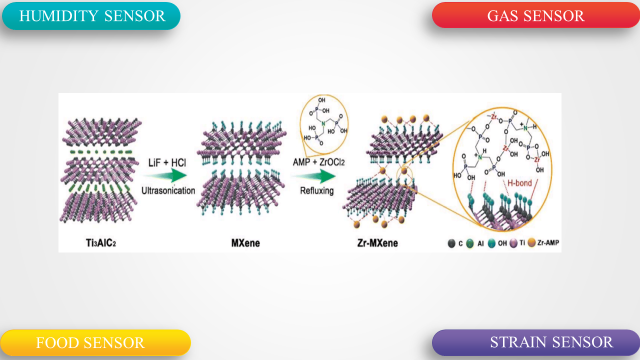
\includegraphics[width=0.72\textwidth]{media/chem2/image12}
	\caption*{Figure 1 - Types of Mxene-based sensors {[}19{]}}
\end{figure}

\begin{table}
\caption*{Table 2 - Advantages and disadvantages of MXepe materials}
\centering
\begin{tblr}{
  row{1} = {c},
  colspec = {X[0.2] X[1] X[1.5]},
  hlines,
  vlines,
}
& \textbf{Advantages} & \textbf{Disadvantages} \\
\textbf{MXene} & {- Stability\\- Optical properties\\- Good hydrophilicity\\- Conductivity\\- Outstanding mechanical properties\\- Thermal effect\\- Excellent biocompatibility\\- High electrical conductivity} & {- The preparation process of MXene sensitive materials must be further developed\\- The abundant functional groups on the surface of MXene materials endow them with customizable optical and electrical properties, but also bring new challenge} 
\end{tblr}
\end{table}

\begin{multicols}{2}
{\bfseries Materials and methods.} \emph{Nanocomposite
WO\textsubscript{3}/Mxene}

Al-Zoha Wapsi and others {[}23{]} used a hydrothermal method
for the synthesis of tungsten oxide nanorods. The synthesis of
WO\textsubscript{3}/MXene by a simple ultrasound method was
carried out. The samples obtained were characterized by
structural, spectral, morphological and elemental analysis. The
photocatalytic and antibacterial activity of synthesized samples,
these aspects are discussed in detail. Max
(Ti\textsubscript{3}AlC\textsubscript{2}) powder was used in a 50
ml Teflon container to synthesize MXene with the formula
Ti\textsubscript{3}C\textsubscript{2}Tx used. To synthesize MXene
with the formula Ti\textsubscript{3}C\textsubscript{2}Tx in a 50 ml
Teflon container. For MXene synthesis, 10 ml of HF is poured
into a Teflon container and then released into a suction cup .
Then, instead of low HF, MAX 0.5 g powder and a pinch were
added. The mixture was equipped with magnetic instruments for
an hour at room temperature.

The combustion optimization of the mixture was carried out at
the installation temperature for 24 hours with magnetic power.
Deionized (DI) water was added to dilute the product, and MXene
was obtained by centrifugation at more than 5000 rpm. The
washing of these deposits was performed until the PH reached 6.
The Aqueous Dispersion was carried out using a PTFE membrane by
vaum filtration. Filtrate is here.

For FESEM analysis, samples were sprayed with gold for 120
seconds at a current of 15 ma. Figure-2 A, B WO\textsubscript{3}
and WO\textsubscript{3}/MXene nanocomposite morphology control.
Figure-2 - (a) illustrates the block/stick pattern morphology of
WO\textsubscript{3}. Figure-2 (b) MXene WO\textsubscript{3} is
defined as impregnated with nano wires. MXene Nano sample
structure formation in Figure 2 - (c). The size of the
WO\textsubscript{3} was about 13 nm, after the reduction of
FESEM. The MXene layer was estimated at \textasciitilde175 nm on
an additional micro-image. For FESEM analysis, the samples were
subjected to gold spraying for 120 seconds at a current of 15
ma. Figure-2 A,B WO\textsubscript{3} and WO\textsubscript{3}/MXene
nanocomposite morphology control. Figure 1 shows the morphology
of WO\textsubscript{3} with a block or stick inscription. Figure -
2 (b) MXene WO\textsubscript{3} is detected in an impregnated
manner with nano wires. Figure 2 (c) shows the MXene formation
of the nanoscale structure. The size of the WO\textsubscript{3}
volume was about 13 nm, which is after the reduction of FESEM.
In the micrograph, the size of the mxen layer was 175 nm.

In this paper, A.Z. Warsi, Aziz, F. Zulfiqar et al. prepared
WO\textsubscript{3}, MXene and WO\textsubscript{3}/MXene
nanocomposite which showed potential applications in biological
and environmental remediation. WO\textsubscript{3}, MXene and
WO/Mxene nanocomposite were synthesized by hydrothermal method,
wet chemical etching and sonication, respectively. XRD, XRD,
FTIR, EDX and FESEM were used to determine the structural,
spectral, elemental and morphological characteristics of the
synthesized samples, respectively. BET analysis was performed to
determine the surface area. The photocatalytic degradation of
methylene blue using WO\textsubscript{3}, MXene and
WO\textsubscript{3}/MXene nanocomposites was 99\%, 54\% and 89\%,
respectively. The photocatalytic activity of WO\textsubscript{3}
was significant. MXene is a two-dimensional material with very
low photocatalytic activity, which acts only as an auxiliary
material to enhance the photocatalytic ability of the composite
with WO\textsubscript{3}.
\end{multicols}

\begin{figure}[H]
	\centering
	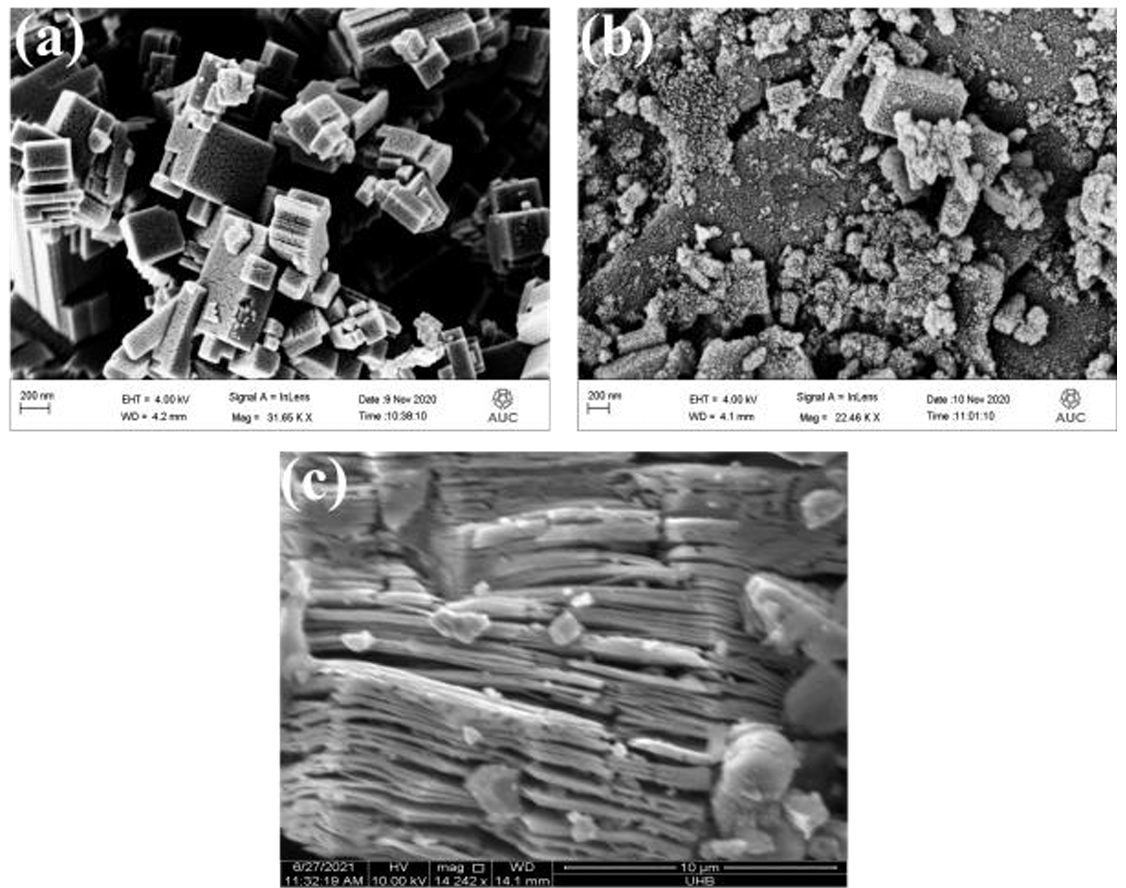
\includegraphics[width=0.9\textwidth]{media/chem2/image13}
	\caption*{Figure 2 - FESEM images (A) WO\textsubscript{3}, (b) WO\textsubscript{3}/MXene nanocomposite and (c) MXene {[}23{]}}
\end{figure}

\begin{multicols}{2}
The prepared samples also showed good antibacterial activity
against bacteria of positive strain; in case of negative strains,
WO\textsubscript{3}, MXene and WO\textsubscript{3}/MXene
nanocomposite showed antibacterial activity at high concentrations
{[}23{]}.

\emph{Bi\textsubscript{2}S\textsubscript{3}/MXene nanocomposite}

In a study {[}24{]} by S. Sinha, A. Raucci et al. developed a
novel electrochemical sensing platform using
Bi\textsubscript{2}S\textsubscript{3}/MXene nanocomposite. The
modified shape, composition and electrical characteristics of the
prepared composites and their electrodes were studied by various
electrochemical methods SEM, XRD, XPS and others. A 1 mg/ml
solution of Bi\textsubscript{2}S\textsubscript{3}/Mxene
nanocomposite was prepared by dispersing DI (deionized) in water.
This standard solution was the base of the electrode
modification process. This initial solution base served as the
electrode modification process. An 8 μL dispersion of
Bi\textsubscript{2}S\textsubscript{3}/Mxene nanocomposites was
carefully placed on the surface of SPE to modify the electrode.
Bi\textsubscript{2}S\textsubscript{3}/Mxene nanocomposites were
synthesized directly by microwave-assisted hydrothermal method.
The figure below shows the accumulation of 3 - (A) {[}24{]}
Bi\textsubscript{2}S\textsubscript{3} nanoparticles. These are
granular nanoparticles with diameters ranging from 70 to 100 nm.
And figure 3 - (B) shows the MXene SPE image. This figure
shows the complex layered lamellar structure of MXene after
removing the Al layers from the MAX phase. SEM image of
Bi\textsubscript{2}S\textsubscript{3}-MXene nanocomposites are
shown in Fig.3C and 3D (small and large scale).
\end{multicols}

\begin{figure}[H]
	\centering
	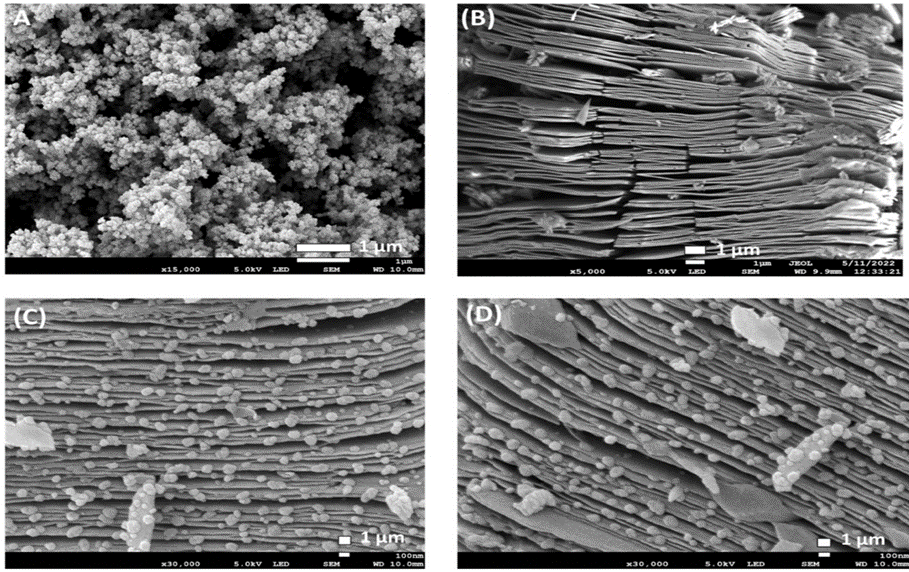
\includegraphics[width=0.9\textwidth]{media/chem2/image14}
	\caption*{Figure 3 - Structural characteristics of (A) Bi\textsubscript{2}S\textsubscript{3}; (B) MXene; (C) Bi\textsubscript{2}S\textsubscript{3}-MXene nanocomposite at low magnification; (D) Bi\textsubscript{2}S\textsubscript{3}-MXene nanocomposite at high magnification {[}24{]}}
\end{figure}

\begin{multicols}{2}
The uniform growth of Bi\textsubscript{2}S\textsubscript{3}
nanoparticles in MXene layers growth of
Bi\textsubscript{2}S\textsubscript{3} nanoparticles (F and OH) was
due to the presence of electronegative functional groups. The
synergistic effect of Bi\textsubscript{2}S\textsubscript{3}
nanoparticles and MXene can improve the electrochemical
performance. First, MXene provides a highly conductive platform
for the uniform growth of Bi\textsubscript{2}S\textsubscript{3}
nanoparticles. This leads to reduced agglomeration of
Bi\textsubscript{2}S\textsubscript{3} nanoparticles and increased
number of detection sites for the target analyte {[}25{]}.
Secondly, MXene is highly conductive, which leads to an increase
in charge between Bi\textsubscript{2}S\textsubscript{3}
nanoparticles and the electrolyte {[}26{]}. In addition, the
oxidation resistance property demonstrated by MXene plays an
important role in protecting Bi\textsubscript{2}S\textsubscript{3}
nanoparticles from corrosion {[}27{]}. The binding of MXene and
Bi\textsubscript{2}S\textsubscript{3} nanoparticles can lead to
improved performance in Zn(II) detection.

\emph{The study focuses on the synthesis of a composite made of
MoO\textsubscript{2}@Mo\textsubscript{2}C-MXene.}

This article discusses the new CdS/MoO\textsubscript{2}
photocatalyst @Mo\textsubscript{2}C-MXene developed by You Jin,
Huizhuan Jing, Libo Wang, Qianku Hu and Aigo Zhou. 0.2 g of
NaBF4 (99.9\%, McLean, China) was used as a guiding reagent,
dissolved in 15 ml of 1.0 m HCl solution (36-38\% C/a , Yantai
Shuangshuang Chemical, China) and stirred for 30 minutes. The
temperature of the hydraulic system is maintained at 180 ℃ for
24 hours every day. The temperature of the hydraulic system is
kept at 180 ℃ for 24 hours every day. Subsequently,
MoO\textsubscript{2}@Mo\textsubscript{2}C-MXene Composite powders
were collected, subjected to washing with deionized water and
ethanol to achieve a neutral reaction, and then dried for 12
hours at 60 ℃ for 12 hours under vacuum conditions.

CdS / MoO\textsubscript{2}@ Mo\textsubscript{2}C photocatalysts
were effectively synthesized by a two-stage hydrothermal method .
In this system, a sediment formed on the surface of the CdS
MoO\textsubscript{2}@Mo\textsubscript{2}C-MXene Composite, forming
an acanthospheric structure. CdS /
MoO\textsubscript{2}@Mo\textsubscript{2}C(CMM5) showed an
exceptional H\textsubscript{2} generation rate of 22,672
µmol/(g-h) in visible light under optimal conditions, which is
11.8 times higher than CdS. full row,
Moo\textsubscript{2}@Mo\textsubscript{2}C-MXene binary co-catalyst
using CdS using high photocatalytic activity of productive
H\textsubscript{2} generation with Mo\textsubscript{2}C MXene as
the only co-catalyst. Experimental effects the
CdS/Mo\textsubscript{2}C system effects work with CdS
/Mo\textsubscript{2}C with high photophysical and
photoelectrochemical properties to serve as an electronic bridge
between CdS and Mo\textsubscript{2}C MXene with improved
electrical conductivity . "no," he said. In addition to the
CdS/Mo\textsubscript{2}C script, the CdS conduction band (CB) is
a place to charge when MoO\textsubscript{2}@Mo\textsubscript{2}C
is MXene bound. This effectively limits the re - diffusion of
Altered electrons into CdS , thus facilitating the operation of
recombination. The band forbidden to control over
CdS/MoO\textsubscript{2}@ Mo\textsubscript{2}C makes it easy to
absorb visible light. This CdS/Mo\textsubscript{2}C {[}28{]}
element restored a new photocatalytic system with the formation
of a binary H\textsubscript{2} co-catalyst.

The process of preparing Ti3C2 involves the use of various
chemical and physical methods to create a highly durable and
efficient material: The crude powder (50 g) was weighed in the
following ratio TiC:Ti:Al = 3.6:1.4:1 and then placed in a
Teflon ball mill. Anhydrous ethanol was then added to the ball
mill tank as a ball grinding aid and zirconium dioxide (5 nm
diameter) as a grinding medium. The mass ratio of raw material
powder, anhydrous ethanol and pellets should be 1:1:3. The
ball was placed in a grinding vessel and the powder mixture
was pulverized at 300 rpm for 4 hours. Next, a ball mill was
used to obtain a homogeneous mixture and then it was transferred
into a petri dish. The mixture was dried in an oven at 40°C for
24 hours, then sintered in a corundum crucible without pressure.

After the reaction was completely completed, the sintering
furnace was allowed to cool down naturally to room temperature
and a Ti\textsubscript{3}AlC\textsubscript{2}
cer\textsubscript{}amic block was obtained by pressureless
sintering. A high-energy ball mill was used to completely
pulverize the Ti\textsubscript{3}AlC\textsubscript{2} ceramic
block obtained by pressureless sintering i+n the previous step;
finally, the desired Ti\textsubscript{3}AlC\textsubscript{2}
powder was successfully obtained. At room temperature, 5 g of
Ti\textsubscript{3}AlC\textsubscript{2} powder was slowly added to
80 mL of 40 wt\% HF and left to react for 24 h under magnetic
stirring at 1200 rpm. The above corrosion products were
purified with deionized water until the pH of the supernatant
became \textgreater{} 6 after centrifugation. The substrate was
lyophilized to obtain Ti\textsubscript{3}C\textsubscript{2} powder.

Preparation of the PANI-Ti\textsubscript{3}C\textsubscript{2}
composite: first, 0.2 g of Ti\textsubscript{3}C\textsubscript{2}
powder was dispersed in 30 mL of 1M hydrochloric acid solution,
then ultrasonic dispersion was carried out for 1 h until a
homogeneous suspension was obtained. Second, 100 μL of pure
aniline (ANI) obtained by distillation was added to the
suspension and dispersed by ultrasonic dispersion for 1h. Then,
0.335 g of ammonium persulfate (APS) was dissolved in 30 mL of 1
M hydrochloric acid solution and added dropwise to the above
solution. Finally, the solution was placed in an ice bath and
stirred at 0°C for 6 hours. After reaction, the reaction product
was washed with ultrapure water 5 times. After purification,
the reaction product was lyophilized to obtain
PANI-Ti\textsubscript{3}C\textsubscript{2} nanocomposite {[}29{]}.

Figure 1A shows the X-ray diffraction patterns of the obtained
PANI, Ti\textsubscript{3}C\textsubscript{2} and
PANI-Ti\textsubscript{3}C\textsubscript{2}. The figure shows that
the X-ray diffraction peak of PANI at 2 theta=20.5° corresponds
to the surface (020) of the PANI crystal. The diffraction peak
of Ti\textsubscript{3}C\textsubscript{2} on the crystal plane
(002) is shifted to the left along the x-axis from that of the
original phase Ti\textsubscript{3}AlC\textsubscript{2}, which
makes the characteristic peak of
Ti\textsubscript{3}C\textsubscript{2} weaker and wider.

This X-ray diffraction pattern can show that the degree of
crystallinity and the degree of structural order of
Ti\textsubscript{3}C\textsubscript{2} are greatly reduced. In the
X-ray radiograph of Ti\textsubscript{3}C\textsubscript{2}, the
diffraction peaks at 2 theta =7.1°, 17°, 28°, 35°, 41° and
61° correspond to the crystal planes (002), (006), (008), (
0010), (0012) and (110), respectively. Compared with the
Ti\textsubscript{3}C\textsubscript{2} XRD, the
PANI-Ti\textsubscript{3}C\textsubscript{2} XRD shows a new
diffraction peak at 2 theta =20.7° corresponding to (020)
crystal surface of PANI. The XRD peak of
PANI-Ti\textsubscript{3}C\textsubscript{2} at 2 theta =26°
corresponds to TiO\textsubscript{2}. This value is due to the
fact that a small amount of Ti\textsubscript{3}C\textsubscript{2}
is oxidized by the addition of ammonium persulfate, an oxidizing
agent, during the preparation of the
PANI-Ti\textsubscript{3}C\textsubscript{2} composite material.
Thus, the phase analysis shows the successful preparation of
PANI-Ti\textsubscript{3}C\textsubscript{2} nanocomposite.
Ti\textsubscript{3}C\textsubscript{2} can easily immobilize
enzymes/proteins on its surface, thus acting as a promising
support to achieve DET with accelerated electrode kinetics, low
detection limits, and high sensitivity and selectivity {[}30{]}.
\end{multicols}

\begin{figure}[H]
	\centering
	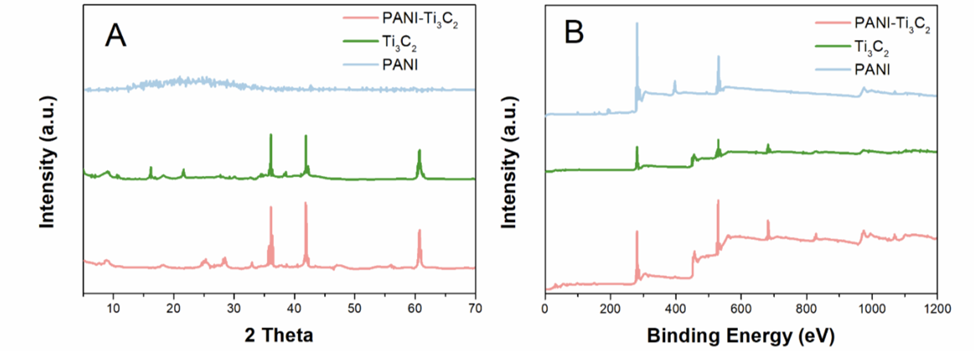
\includegraphics[width=0.9\textwidth]{media/chem2/image15}
	\caption*{Figure 4 - (A) XRD patterns of PANI, Ti\textsubscript{3}C\textsubscript{2} and PANI-Ti\textsubscript{3}C\textsubscript{2}. (B) XPS spectras of PANI, Ti\textsubscript{3}C\textsubscript{2} and PANI-Ti\textsubscript{3}C\textsubscript{2} {[}30{]}}
\end{figure}

\begin{multicols}{2}
Figure 1B shows the XRD spectra of the obtained PANI,
Ti\textsubscript{3}C\textsubscript{2} and
PANI-Ti\textsubscript{3}C\textsubscript{2}. As can be seen from
the figure, characteristic peaks C1s, O1s, F1s and
Ti\textsubscript{2}p appear, proving the existence of
Ti\textsubscript{3}C\textsubscript{2}. At the same time, the
appearance of characteristic peaks O1s and F1s proves the
existence of functional groups -O, -OH and -F on the laminates of
Ti\textsubscript{3}C\textsubscript{2}. The appearance of C1s and
N1s peaks indicates the successful obtaining of PANI. Compared
with Ti\textsubscript{3}C\textsubscript{2} , the broad XPS
spectrum of PANI-Ti\textsubscript{3}C\textsubscript{2} shows N1s
peak, which further proves the successful preparation of
PANI-Ti\textsubscript{3}C\textsubscript{2} nanocomposites under
low temperature stirring conditions. The above results are in
agreement with the results of X-ray diffraction analysis. By the
integral approximation method, N1s -analysis of the RFES spectra
of the PANI-Ti\textsubscript{3}C\textsubscript{2}
nan\textsubscript{}ocomposite showed four characteristic peaks at
397.1 eV, 398.2 eV, 400.1 eV and 400.5 eV corresponding to the
imine structure (=NH-), amino group (-NH-). -), N atom (N-+) with
positron and protonated amino group, respectively. The results
show that the PANI-Ti\textsubscript{3}C\textsubscript{2}
nanocomposite was successfully obtained by low-temperature
oxidation reaction between Ti\textsubscript{3}C\textsubscript{2}
and aniline.

\emph{Ti\textsubscript{3}C\textsubscript{2}/TiO\textsubscript{2}/CuO
nanocomposites}

In experiments, researchers Li, Wang, and Sun dissolved copper
nitrate in deionized water and added
Ti\textsubscript{3}C\textsubscript{2} powder. The mixture was
incubated for 24 hours, dried, and then synthesized into
Ti\textsubscript{3}C\textsubscript{2}/TiO\textsubscript{2}/CuO
nanocomposites by annealing in an argon atmosphere at 500C for 30
minutes at a heating rate of 100C/min {[}31{]}. \hl{}

The fabrication of
Ti\textsubscript{3}C\textsubscript{2}/TiO\textsubscript{2}/CuO
ternary nanocomposites, consisting of
Ti\textsubscript{3}C\textsubscript{2} nanosheets,
TiO\textsubscript{2}, and CuO nanoparticles, was enhanced by
higher electron and hole separation efficiency compared to
TiO\textsubscript{2}, thereby improving their photocatalytic
activity {[}32{]}.

{\bfseries Discussion and results.} In this research, a series of
MXene-based nanocomposites including WO\textsubscript{3}/MXene,
Bi\textsubscript{2}S\textsubscript{3}/MXene, and
Ti\textsubscript{3}C\textsubscript{2}/TiO\textsubscript{2}/CuO were
synthesized and characterized. The obtained materials showed
high efficiency in various applications including photocatalytic
decomposition of organic pollutants and electrochemical detection
of heavy metals.

WO\textsubscript{3}/MXene:

- The morphology of the nanocomposite determined by FESEM revealed
the presence of nanowires and layered structure.

- The photocatalytic activity for methylene blue degradation
reach-ed 89\%, which is higher than that of pure
WO\textsubscript{3} (99\%) and significantly superior to that of
MXene (54\%).

- The nanocomposite demonstrated antibacterial activity against
both positive and negative bacterial strains at high
concentrations.

Bi\textsubscript{2}S\textsubscript{3}/MXene:

- The synergistic effect of Bi\textsubscript{2}S\textsubscript{3}
and MXene was found to improve electrochemical performance,
increase the number of active sites for analytical detection,
and improve corrosion resistance.

- The nanocomposite was successfully used for Zn(II) detection
with high sensitivity.

Ti\textsubscript{3}C\textsubscript{2}/TiO\textsubscript{2}/CuO:

- The ternary nanocomposite showed enhanced photocatalytic
activity due to the improved electron-hole separation ability.

- The enhanced photocatalytic efficiency was attributed to the
presence of TiO\textsubscript{2} and CuO, which enhanced the
interaction with Ti\textsubscript{3}C\textsubscript{2}.

These results confirm the potential of MXene-based nanomaterials
in applications related to ecological remediation, biosensing and
environmental monitoring.

The results confirm the significant contribution of MXene-based
nanocomposites in improving the properties of sensors and
catalysts.

\emph{Photocatalytic activity:}

The high efficiency of WO\textsubscript{3}/MXene in the
photocatalytic decomposition of methylene blue can be explained by
the combination of MXene (high conductivity) and
WO\textsubscript{3} (active catalytic ability) properties. This
supports the hypothesis of a synergistic effect in the creation
of hybrid nanomaterials. Similarly,
Ti\textsubscript{3}C\textsubscript{2}/TiO\textsubscript{2}/CuO
nanocomposite demonstrates that the addition of CuO enhances the
charge separation ability, which is critical for photocatalysis.

\emph{Electrochemical detection:}

Bi\textsubscript{2}S\textsubscript{3}/MXene showed high sensitivity
to Zn(II), which is attributed to the increase of active centers
on the surface of MXene and its interaction with
Bi\textsubscript{2}S\textsubscript{3}. This result is in line with
current research in electrochemistry, where MXene is used as a
basic structure to improve the sensor response.

\emph{Lim}\emph{itations and prospects:}

Despite significant advances, difficulties in scaling up the
production of MXene nanocomposites should be considered.
Additional research is required to optimize synthesis methods and
material stability. Prospects for the use of these materials
include expanding their applications in environmental monitoring,
biomedicine, and water quality control.

Thus, the results of this study confirm the relevance and
promise of MXene-based nanocomposites for the development of
high-performance sensors and catalysts. Future research should
focus on improving the stability and fabrication processes of
these materials.

{\bfseries Conclusion.} This literature review is devoted to the
detection of heavy metals. Heavy metals are found in many
substances. There are many methods for detecting heavy metals.
Despite the large number of methods, we must use the most
effective of them. The article is written about the detection of
heavy metals using a sensor. In order to improve the sensor,
various nanomaterials are used. As a material, Mxene-based
nanocompasites were considered. Focused on MXene-based
nanocomposites and sensor research methods developed on their
basis. MXene materials are a stable single-phase structure
consisting of five or more atoms, and its elemental ratio can
be adjusted. MXene contains more transition metals, which
greatly optimizes material properties such as conductivity,
hardness, chemical stability, and bulk capacity.
\end{multicols}

\begin{center}
{\bfseries References}
\end{center}

\begin{references}
1. Singovszka E., Balintova M., Junakova N. The Impact of Heavy
Metals in Water from Abandoned Mine on Human Health//SN Applied
Sciences.-2020.-Vol.2:934

 DOI 10.1007/s42452-020-2731-2

2. Munir N., Jahangeer M., Bouyahya A., El Omari N., Ghchime R.,
Balahbib A., Aboulaghras S., Mahmood Z., Akram M., Ali Shah S.M.
Heavy Metal Contamination of Natural Foods Is a Serious Health
Issue: A Review//Sustainability.-2022.-Vol.14(1),161.
\href{https://doi.org/10.3390/su14010161}{DOI 10.3390/su14010161}

3. Ali H., Khan E. Trophic Transfer, Bioaccumulation, and
Biomagnification of Non-Essential Hazardous Heavy Metals and
Metalloids in Food Chains/Webs-Concepts and Implications for
Wildlife and Human Health//Human and Ecological Risk
Assessment.-2018.-Vol. 25(6).-P.1353-1376
\href{https://doi.org/10.1080/10807039.2018.1469398}{DOI\\
10.1080/10807039.2018.1469398}

4. Kumari P., Chowdhury A., Maiti S.K. Assessment of Heavy Metal
in the Water, Sediment, and Two Edible Fish Species of
Jamshedpur Urban Agglomeration, India with Special Emphasis on
Human Health // Human and Ecological Risk
Assessment.-2018.-Vol.24(7).-P.1-24
\href{https://doi.org/10.1080/10807039.2017.1415131}{DOI\\
10.1080/10807039.2017.1415131}

5. Sharma S., Nagpal A.K., Kaur I. Appraisal of Heavy Metal
Contents in Groundwater and Associated Health Hazards Posed to
Human Population of Ropar Wetland, Punjab, India and its
Environs // \\Chemosphere.-2019.-Vol. 227.- P.179 - 190.
\href{https://doi.org/10.1016/j.chemosphere.2019.04.009}{DOI
10.1016/j.chemosphere.2019.04.009}

6. Cheng S. Heavy metal pollution in China: Origin, pattern and
control// Enviro nmental Science

and Pollution Research.-2003.-Vol.10.-P.192-198.
\href{https://doi.org/10.1065/espr2002.11.141.1}{DOI
10.1065/espr2002.11.141.1}

7. Zykova I., Maksimuk N., Rebezov M., Kuznetsova E., Derkho M.,
Sereda T., Kazhibayeva G., Somova Y., Zaitseva T. Interaction
between Heavy Metals and Microorganisms during Wastewater
Treatment by Activated Sludge//ARPN Journal of Engineering and
Applied Sciences.-2020.-Vol.14(11).- P.2139--2145(2019).

8. Maria J.da Silva M, Paim A.P., I., Pimentel M.F., Cervera M.L.,
de la Guardia M. Determination of TOtal Mercury in Spanish Samples
of Baby Food, Fast Food, and Daily Meal//Journal of the
Brazilian Chemical Society.-2023.-Vol.34(4).-P.517-526.
\href{http://dx.doi.org/10.21577/0103-5053.20220125}{DOI
10.21577/0103-5053.20220125}

9. Qin G., Niu Z., Yu J., Li Z., Ma J., Xiang P. Soil heavy
metal pollution and food safety in China: Effects, sources and
removing technology//Chemosphere.-2021.-Vol.267:129205
\href{https://doi.org/10.1016/j.chemosphere.2020.129205}{DOI\\
10.1016/j.chemosphere.2020.129205}

10. Liliana A.N., Gheorghe G., Elena T., Sonia A. Electrochemical
sensors and biosensors: effective tools for detecting heavy
metals in water and food with possible implications for
children's health//International Journal of Electrochemical
Science, 19(2024).
\href{https://doi.org/10.1016/j.ijoes.2024.100643}{DOI
10.1016/j.ijoes.2024.100643}

11. Baranwal J., Barse B., Gatto G., Broncova G., Kumar A.
Electrochemical Sensors and Their \\Applications: A
Review//Chemosensors.-2022.-Vol.10(9):363.
\href{https://doi.org/10.3390/chemosensors10090363}{DOI
10.3390/chemosensors10090363}

12. Sammer-ul H., Zhang X. Microfluidics as an emerging platform
for tackling antimicrobial resistance (AMR): a review// Current
Analytical Chemistry.-2020.-Vol.16 (1).-P. 41-51
DOI \\10.2174/1573411015666181224145845

13. Pohanka M. Screen printed electrodes in biosensors and
bioassays. A review// International Journal of Electrochemical
Science.-2020.-Vol.15 (11).-P.11024-11035.
DOI 10.20964/2020.11.19

14. Ozcelikay G., Karadurmus L., Kaya S.I., Bakirhan N.K., Ozkan
S.A. A review: new trends in electrode systems for sensitive
drug and biomolecule analysis// Critical Reviews in Analytical
Chemistry.-2020.-Vol.50(3).-P. 212-225(2020). DOI
10.1080/10408347.2019.1615406

15. Wang X., Kong L., Zhou S., Ma C., Lin W., Sun X., Kirsanov
D., Legin A.,. Wan H, Wang P. Development of QDs-based nanosensors
for heavy metal detection: a review on transducer principles and
in-situ detection// Talanta.- 2022.-Vol.239. DOI
\href{https://doi.org/10.1016/j.talanta.2021.122903}{10.1016/j.talanta.2021.122903}

16. Shenashen M.A., Emran M.Y., El Sabagh A., Selim M.M.,
Elmarakbi A.,. El- Safty S.A. Progress in sensory devices of
pesticides, pathogens, coronavirus, and chemical additives and
hazards in food assessment: food safety concerns//Progress in
Materials Science.-2020.-Vol. 124 DOI\\
\href{http://dx.doi.org/10.1016/j.pmatsci.2021.100866}{10.1016/j.pmatsci.2021.100866}

17. Huang W., Hu L., Tang Y., Xie Z., Zhang H. Recent Advances in
Functional 2D MXene-Based Nanostructures for Next Generation
Devices// Adv. Funct. Mater.- 2020.- Vol.30 (49).
DOI \\10.1002/adfm.202005223

18. Zhou L., Zhang X., Ma L., Gao J., Jiang Y. Acetylcholinester
ase/chitosan-transition metal carbides nanocomposites-based bio
sensor for the organophosphate pesticides detection// Biochem.
Eng. J.-2017.-Vol.128. P.243-249.
\href{https://doi.org/10.1016/j.bej.2017.10.008}{DOI
10.1016/j.bej.2017.10.008}

19. Hossein R., Golnoush T., Masoud S. MXene-Based Nanocomposite
Sensors// ACS Omega.-2021.-Vol. Vol.6(17).-
P.11103-11793\href{https://pubs.acs.org/doi/10.1021/acsomega.0c05828}{.
DOI /10.1021/acsomega.0c05828}

20. Garcia-Miranda Ferrari A., Carrington P., Rowley-Neale S.J.,
Banks C.E. Recent advances in portable heavy metal
electrochemical sensing platforms, Envi- ron// Environmental
Science: Water Research \& Technology.-2020.-Vol. 6 (10).-
P.2676-2690.DOI 10.1039/D0EW00407C

21. Amtul N., Kulamani P. A Glimpse on the plethora of
applications of prodigious material MXene // Sustainable Materials
and Technologies.-2022.-Vol.32: e00439
\href{https://doi.org/10.1016/j.susmat.2022.e00439}{DOI
10.1016/j.susmat.2022.e00439}

22. Aadil M., Zulfiqar S., Shahid M., Haider S., Shakir I.,
Warsi M.F. Binder free mesoporous Ag-doped Co3O4 nanosheets with
outstanding cyclic stability and rate capability for advanced
supercapacitor applications//Journal of Alloys and
Compounds.-2020.-Vol.844:156062

\href{https://doi.org/10.1016/j.jallcom.2020.156062}{DOI
10.1016/j.jallcom.2020.156062}

23. Warsi A.-Z., Aziz F., Zulfiqar S., Haider S., Shakir I.,
Agboola P.O. Synthesis, Characterization, Photocatalysis, and
Antibacterial Study of WO3, MXene and WO\textsubscript{3}/MXene
Nanocomposite//\\ Nanomaterials .-2022.-Vol.12(4): 713 DOI
\href{http://dx.doi.org/10.3390/nano12040713}{10.3390/nano12040713}

24.Sima S., Ada R., Wanda C., Arshid N., Mohammad K., Stefano C.
Bismuth-MXene nanocomposite: A low-cost portable solution for
zinc (II) detection in water for safer environmental
monitoring//Sensors and Actuators B: Chemical.-2024. Vol
418:136219.
\href{https://doi.org/10.1016/j.snb.2024.136219}{DOI\\
10.1016/j.snb.2024.136219}

25. Iqbal M.A., Tariq A., Zaheer A., Gul S., Ali S.I., Iqbal
M.Z., Akinwande D., Rizwan S.
Ti\textsubscript{3}C\textsubscript{2}-MXene/bismuth ferrite
nanohybrids for efficient degradation of organic dyes and
colorless pollutants//ACS Omega.-2019.-Vol. 4(24)-P.20530-20539.
\href{https://doi.org/10.1021/acsomega.9b02359}{DOI
10.1021/acsomega.9b02359}

26. Palei S., Murali G., Kim C.H., In I., Lee S.Y., Park S.J. A
review on interface engineering of MXenes for perovskite solar
cells//Nano-Micro Lett.-2023.-Vol.15(1):123
\href{https://doi.org/10.1007/s40820-023-01083-9}{DOI
10.1007/s40820-023-01083-9}.

27. Gogotsi Y., Anasori B. The Rise of MXenes//ACS
Nano.-2019.-Vol.13(8).-P. 8491-8494.
\href{https://doi.org/10.1021/acsnano.9b06394}{DOI\\
10.1021/acsnano.9b06394}.

28. Sen J., Huijuan J., Libo W., Qianku H., Aiguo Z. Construction
and performance of
CdS/MoO\textsubscript{2}@Mo\textsubscript{2}C-MXene photocatalyst
for H\textsubscript{2} production// Journal of Advanced
Ceramics.-2022.- Vol.11. -P.1431- 1444.
\href{https://doi.org/10.1007/s40145-022-0621-3}{DOI
10.1007/s40145-022-0621-3}.

29. Haoliang C., Jurui Y. Preparation of
Ti\textsubscript{3}C\textsubscript{2}-PANI Composite as Sensor for
Electrochemical \\Determination of Mercury Ions in
Water//International Journal of Electrochemical Science.-2020.-\\
Vol.15(3).-P. 2295 -- 2306. DOI 10.20964/2020.03.24

30. Sinha A., Dhanjai, Zhao H., Huang Y., Lu X., Chen J., Jain R.
MXene: An emerging material for sensing and biosensing//TrAC
Trends in Analytical Chemistry.-2018.-Vol.105.-P. 424-435 DOI\\
\href{http://dx.doi.org/10.1016/j.trac.2018.05.021}{10.1016/j.trac.2018.05.021}

31. Li Z.Y., Wang L.B., Sun D.D. Synthesis and thermalstability
of two-dimensional carbide MXene
Ti\textsubscript{3}C\textsubscript{2}//\href{https://www.researchgate.net/journal/Materials-Science-and-Engineering-B-0921-5107?_tp=eyJjb250ZXh0Ijp7ImZpcnN0UGFnZSI6InB1YmxpY2F0aW9uIiwicGFnZSI6InB1YmxpY2F0aW9uIn19}{Materials
Science and Engineering} B- 2015.-Vol.191.- P.33-40.
DOI \href{http://dx.doi.org/10.1016/j.mseb.2014.10.009}{10.1016/j.mseb.2014.10.009}

32. Yang L., Meihuan Y., Aiguo Z., Qianku H., Libo W.
Preparation and Photocatalytic Performance of
Ti\textsubscript{3}C\textsubscript{2}/TiO\textsubscript{2}/CuO
Ternary Nanocomposites// Journal of Nanomaterials.-2017.-Vol.2017.
P.1-5 DOI 10.1155/2017/1978764
\end{references}

\begin{authorinfo}
\emph{{\bfseries Information about the authors}}

Konarbay D.B. {\bfseries -} Doctoral student at the Kazakh National
Pedagogical University named after Abay, Almaty, Kazakhstan,e-mail:
\href{mailto:konarbay98@bk.ru}{\nolinkurl{konarbay98@bk.ru}};

Bakytkarim Y. {\bfseries -} Doctor Ph.D, Abai Kazakh National
Pedagogical University, Almaty, Kazakhstan, e-mail:\\
\href{mailto:Rysgul_01_88@mail.ru}{\nolinkurl{Rysgul\_01\_88@mail.ru}};

Mukatayeva Zh.- Can{\bfseries }didate of Chemical Sciences, Associate
Professor, Abai Kazakh National Pedagogical University, Almaty,
Kazakhstan, e-mail:
\href{mailto:zh.mukatayeva@abaiuniversity.edu.kz}{\nolinkurl{zh.mukatayeva@abaiuniversity.edu.kz}};

Shadin N.A {\bfseries -} Doc{\bfseries }tor Ph.D, Senior Lecturer of the
Department of Chemistry, Abai Kazakh National Pedagogical
University, Almaty, Kazakhstan, e-mail: nugen\_87@mail.ru;

Kozhagulova Zh.R. {\bfseries -} Senior Lecturer of the Department of
Chemistry, Abai Kazakh National Pedagogical University, Almaty,
Kazakhstan, e-mail:
\href{mailto:karazhanova71@mail.ru}{\nolinkurl{karazhanova71@mail.ru}};

Karazhanova D.A. {\bfseries -} Senior Lecturer of the Department of
Chemistry, Abai Kazakh National Pedagogical University, Almaty,
Kazakhstan, e-mail:
\href{mailto:Kozhagulova.zh@gmail.com}{\nolinkurl{Kozhagulova.zh@gmail.com}}

\emph{{\bfseries Сведения об авторах}}

Конарбай Д.Б.-- докторант Казахский Национальный Педагогического им.
Абая, Алматы, Казахстан, e-mail:\\
\href{mailto:konarbay98@bk.ru}{\nolinkurl{konarbay98@bk.ru}};

Бакыткарим Ы{\bfseries .} -- доктор PhD, старший преподаватель
кафедры химии Казахского национального педагогического
университета им. Абая, Алматы, Казахстан. e-mail:
\href{mailto:Rysgul_01_88@mail.ru}{\nolinkurl{Rysgul\_01\_88@mail.ru}};

Мукатаева Ж.С.-- кандидат химических наук, ассоциированный
профессор, заведующий кафедрой химии Казахского национального
педагогического университета им. Абая, Алматы, Казахстан. e-mail:
\href{mailto:zh.mukatayeva@abaiuniversity.edu.kz}{\nolinkurl{zh.mukatayeva@abaiuniversity.edu.kz}};

Шадин Н.А.-- доктор PhD, старший преподаватель кафедры химии
Казахского национального педагогического университета им. Абая,
Алматы, Казахстан. e-mail: nugen\_87@mail.ru;

Кожагулова Ж.Р. - старший преподаватель кафедры химии Казахского
национального педагогического университета им. Абая, Алматы,
Казахстан. e-mail:
\href{mailto:karazhanova71@mail.ru}{\nolinkurl{karazhanova71@mail.ru}};

Каражанова Д.А. старший преподаватель кафедры химии Казахского
национального педагогического университета им. Абая, Алматы,
Казахстан. e-mail:
\href{mailto:Kozhagulova.zh@gmail.com}{\nolinkurl{Kozhagulova.zh@gmail.com}}
\end{authorinfo}
